\documentclass[portuguese]{textolivre}

% metadata
\journalname{Texto Livre}
\thevolume{17}
%\thenumber{1} % old template
\theyear{2024}
\receiveddate{\DTMdisplaydate{2024}{3}{11}{-1}}
\accepteddate{\DTMdisplaydate{2024}{6}{10}{-1}}
\publisheddate{\today}
\corrauthor{Maria Elisa Rodrigues Moreira}
\articledoi{10.1590/1983-3652.2024.51574}
%\articleid{NNNN} % if the article ID is not the last 5 numbers of its DOI, provide it using \articleid{} commmand 
% list of available sesscions in the journal: articles, dossier, reports, essays, reviews, interviews, editorial
\articlesessionname{articles}
\runningauthor{Moreira e Ferraz}
%\editorname{Leonardo Araújo} % old template
\sectioneditorname{Daniervelin Pereira}
\layouteditorname{João Mesquita}

\title{A multimodalidade na literatura para crianças e jovens e suas experimentações estéticas e digitais}
\othertitle{Multimodality in literature for children and young people and its aesthetic and digital experimentation}

\author[1]{Maria Elisa Rodrigues Moreira~\orcid{0000-0002-2177-7762}\thanks{Email: \href{mailto:elisarmoreira@gmail.com}{elisarmoreira@gmail.com}}}
\author[2]{Bruna Fontes Ferraz~\orcid{0000-0002-9136-6838}\thanks{Email: \href{mailto:bruna.fferraz@gmail.com}{bruna.fferraz@gmail.com}}}
\affil[1]{Universidade Presbiteriana Mackenzie, Programa de Pós-Graduação em Letras, Letras, São Paulo, SP, Brasil.}
\affil[2]{Centro Federal de Educação Tecnológica de Minas Gerais, Programa de Pós-Graduação em Estudos de Linguagens, Departamento de Linguagem e Tecnologia, Belo Horizonte, MG, Brasil.}

\addbibresource{article.bib}

\usepackage{soul}

\begin{document}
\maketitle
\begin{polyabstract}
\begin{abstract}
Este artigo aborda a pluralidade e expansão da literatura contemporânea,
especialmente daquela produzida para crianças e jovens, na qual a
experimentação estética é proeminente, seja pelas potencialidades da linguagem
verbal, seja pelas possibilidades materiais do objeto livro. Explorando o
conceito de literatura em campo expandido e sua relação com a multimodalidade,
o texto analisa três obras: \textit{A queda dos moais}, de Blandina Franco,
Patricia Auerbach e José Carlos Lollo; \textit{Sinfonia dos animais}, de Dan
Brown; e a série \textit{Mobeybou}. Essas obras exemplificam diferentes
abordagens na utilização da multimodalidade e da intermidialidade, desde
aquelas que não recorrem a tecnologias digitais até aquelas que se apoiam
fortemente nelas. A análise visa compreender como essas estratégias estéticas e
tecnológicas impactam a experiência do leitor jovem. O texto está estruturado
em quatro seções, além da introdução e das considerações finais, que discutem a
relação entre multimodalidade, literatura em campo expandido e tecnologia na
produção literária contemporânea.

\keywords{Multimodalidade \sep Literatura em campo expandido \sep Literatura para crianças e jovens \sep Intermidialidade}
\end{abstract}

\begin{english}
\begin{abstract}
This article discusses the plurality and expansion of contemporary literature,
especially the one produced for children and young people, in which aesthetic
experimentation is prominent, both through the potential of verbal language and
the material possibilities of the book object. Exploring the concept of
literature in the expanded field and its relationship with multimodality, the
text analyses three works: \textit{A queda dos moais} (\textit{The fall of the
moai}, in free translation), by Blandina Franco, Patricia Auerbach and José
Carlos Lollo; \textit{Wild symphony}, by Dan Brown; and the \textit{Mobeybou}
series. These works exemplify different approaches to the use of multimodality
and intermediality, from those that do not use digital technologies to those
that rely heavily on them. The analysis aims to understand how these aesthetic
and technological strategies impact on the young reader's experience. The text
is structured in four sections, in addition to the introduction and final
considerations, which discuss the relationship between multimodality,
literature in the expanded field and technology in contemporary literary
production.

\keywords{Multimodality \sep Literature in the expanded field \sep Literature for Children and Young People \sep Intermediality}
\end{abstract}
\end{english}
\end{polyabstract}

\section{Introdução}

A literatura contemporânea se caracteriza pela pluralidade de formas pelas
quais é produzida, posta em circulação e consumida, assim como por sua
variabilidade estética: o material é tão diverso que, muitas vezes, torna-se
difícil identificar o que é um livro e o que não é, o que é literatura e o que
não é. Nesses espaços plurais, as fronteiras entre os objetos estéticos e
culturais tornam-se cada vez mais espessas e, ao mesmo tempo, mais porosas,
funcionando mais como territórios de diálogo e transição que como limites
circunscritores \cite{hissa_mobilidade_2006}.

Nesse cenário, tem ganhado espaço nas discussões atinentes aos estudos
literários aquelas que refletem sobre a chamada literatura em campo expandido,
expressão que remete justamente a esse cenário no qual a identificação do que
seria específico do literário se torna algo cada vez mais indefinido. Oriunda
de debates no campo do cinema \cite{youngblood_expanded_1970} e das artes
plásticas \cite{krauss_escultura_2008}, a expressão estabeleceu seu diálogo com
a literatura por meio, em especial, das reflexões de pesquisadoras como
\textcite{ludmer2010literaturas} e \textcite{garramuno_frutos_2014}, que vêm discutindo,
respectivamente, o que denominam como pós-autonomia da literatura e
inespecificidade das artes.

A produção literária voltada às crianças e aos jovens
\cite{hunt_critica_2010,zilberman_como_2005} não fica de fora deste cenário de
expansão, sendo talvez um dos campos nos quais as experimentações estéticas são
mais exploradas, seja pelas potencialidades da linguagem verbal, seja pelas
possibilidades materiais do objeto livro, no qual essa literatura
prioritariamente circula. Um exemplo claro são as inúmeras pesquisas que
envolvem os livros ilustrados endereçados a essa faixa etária, as quais apontam
para o potencial estético, poético e narrativo dessas obras, que demandam um
olhar diferenciado da crítica \cite{linden_para_2011}.

Neste artigo, interessa-nos pensar especialmente em como essa expansão se
realiza, em determinadas obras, pelo recurso à multimodalidade, que permite
expressões criativas bastante distintas entre si. Para tanto, destacamos três
obras que nos interessam explorar em seus aspectos estéticos, observando de que
modo elas se valem de diferentes estratégias para apresentar aos seus jovens
leitores narrativas interessantes e informativas formadas a partir de distintas
linguagens.

Para o desenvolvimento do artigo, o estruturamos em quatro seções, além desta
Introdução e das Considerações finais. Na \Cref{sec-normas}, discutiremos a
questão da multimodalidade e de sua interpolação com os estudos sobre a
literatura em campo expandido. Na terceira, abordamos o livro \textit{A queda dos
moais}, de Blandina Franco, Patricia Auerbach e José Carlos Lollo, lançado em
2018, uma obra que trabalha a multimodalidade sem recorrer a tecnologias
digitais ou à intermidialidade. Na quarta seção analisamos o livro \textit{Sinfonia dos
animais}, de Dan Brown, publicado em 2020, que propõe uma experiência
multissensorial ao ser acompanhado de músicas acessadas por meio de um
aplicativo de realidade aumentada, ou seja, um livro para ler e ouvir, com o
acompanhamento de outro aparelho, o celular. Na quinta seção, investigamos um
produto cujo foco é a exploração das possibilidades interativas das tecnologias
digitais, sendo ora classificado como um \textit{app book}, ora como um game: trata-se
da série em quatro volumes \textit{Mobeybou}, composta pelos títulos \textit{Mobeybou na Índia},
\textit{Mobeybou em Cabo Verde}, \textit{Mobeybou no Brasil} e \textit{Mobeybou em Portugal}. Por fim,
apresentamos nossas considerações em torno da pluralidade de usos da
multimodalidade nas obras analisadas.

\section{Multimodalidade e literatura em campo expandido: interpolações}\label{sec-normas}

Para representar o mundo que o cerca, o homem recorre a diferentes linguagens,
que lhe permitem compreendê-lo e abarcá-lo. Diante da complexidade dos eventos
externos, o registro simbólico parece, por vezes, limitado ou insuficiente, de
forma que recorrer à pluralidade de \textit{modos} ou \textit{meios} de
representação torna-se uma estratégia eficaz. Fenômeno, portanto, antigo,
embora a nomenclatura possa ser considerada relativamente recente\footnote{
    Como destaca Ruth Page na introdução ao livro \textit{New Perspectives on Narrative
    and Multimodality}, é apenas a partir dos anos 1990 que o conceito de
    multimodalidade passa a interessar criticamente a estudos das mais diversas
    áreas, capitaneados em especial pelo trabalho do New London Group, um grupo de
    pesquisa acadêmica norte-americano que se volta aos multiletramentos
    \cite[p.~3-5]{page_new_2010}.},
a \textit{multimodalidade} constitui, em
essência, todo texto que reivindica outros \textit{modos}, ou outras
\textit{mídias}, como as imagens, por exemplo, em sua constituição. A esse
respeito, \textcite{vieira_multimodalidade_2015}, recorrendo à Teoria da
Multimodalidade do Discurso, observa que:
\begin{quote}
    [...] se os seres humanos produzem e comunicam significações em vários
    modos semióticos, então somente o uso da linguagem verbal se tornaria
    insuficiente para concentrar a atenção de quem está interessado na produção
    e na reprodução social de significados. Logo, se, em essência, os textos
    são multimodais, será impossível ler significados representados apenas por
    um modo linguístico \cite[p.~44]{vieira_multimodalidade_2015}.
\end{quote}

Alguns pesquisadores, como destaca \textcite{page_new_2010}, apontam que a
multimodalidade constitui, por excelência, o modo como nos comunicamos, uma vez
que sempre recorremos à integração de múltiplos recursos semióticos para tal.
Isso implicaria a necessidade de que repensemos o destaque que, tanto teórica
quanto metodologicamente, damos aos recursos verbais no conjunto de
configurações semióticas múltiplas, e nos demandaria movimentos de investigação
das narrativas em que valorizássemos outros recursos com a mesma dedicação.

Essa combinação de semioses, que está, assim, no cerne da produção de discursos
e de sentidos, tem sido ainda mais evidenciada após a democratização do acesso
às tecnologias digitais e eletrônicas, que expandiram as possibilidades de
interação com o real, passando, inclusive, a simulá-lo ou rivalizá-lo. Ao
ampliar os \textit{modos} de produção textual, estimulando cada vez mais outras
percepções sensoriais, a ascensão das tecnologias digitais parece ter
complexificado o próprio sentido de \textit{multimodalidade}.
\textcite{ellestrom_modalities_2021} observa que: “No contexto dos estudos de
mídia e linguística, ‘multimodalidade’, às vezes, se refere à combinação,
digamos, de texto, imagem e som, e, às vezes, à combinação das faculdades
sensoriais (auditiva, visual, tátil e assim por diante).”. O autor sueco parece
destacar a exploração sensorial para a classificação de tal fenômeno quando
conclui: “Portanto, a multimodalidade foi definida como ‘o uso de dois ou mais
dos cinco sentidos para a troca de informações’ (Granström et al. 2002: 1).”
\cite[p.~41, tradução nossa]{ellestrom_modalities_2021}\footnote{
    No original:
    “In the context of media studies and linguistics, ‘multimodality’ sometimes
    refers to the combination of, say, text, image and sound, and sometimes to the
    combination of sense faculties (the auditory, the visual, the tactile and so
    forth). Thus, multimodality has been defined as ‘the use of two or more of the
    five senses for the exchange of information’ (Granström et al. 2002: 1).”}.

Se concordarmos com o pesquisador sueco, o texto multimodal, ao conclamar
outros \textit{modos} de representação, como a imagem, o som, o papel, a tela e
assim por diante, estaria aproximando diferentes artes e tecnologias para
aguçar ou estimular os sentidos do leitor, e essa seria sua característica
constitutiva. Nas palavras de \textcite[p.~100]{gibbons_i_2010}, “os romances
multimodais, em sua utilização de múltiplos estímulos sensoriais, são
conscientes de sua forma material, explorando a natureza integrativa da
cognição e a natureza corporificada da leitura”\footnote{No original: “[…]
multimodal novels in their employment of multiple sensory stimuli are
self-conscious of their material form, playing upon the integrative nature of
cognition and embodied nature of reading.”.}.

A literatura, portanto, ao convidar outros \textit{modos} e \textit{mídias}
para dividirem o espaço do texto e com o texto, por meio de um processo lúdico
e tangível, estimula o aprendizado e a produção de saberes. Se essa intenção
sempre esteve presente no panorama da produção literária, sobretudo para
crianças e jovens, com as tecnologias outros recursos passam a ser incorporados
ao processo criativo, contribuindo ainda mais com a construção simbólica,
imaginativa e ficcional.

A abertura do texto, do discurso e, em última instância, da própria literatura
aos outros campos artísticos evidencia um processo de aproximação e
distanciamento, de atração e repulsão, de convergência e divergência, que
culmina em formas estéticas que, de algum jeito, em positivo ou em negativo,
são construídas a partir dessas marcas, desses vestígios, dessas ruínas
estabelecidas pelo contato. Da multimodalidade à literatura em campo expandido,
entramos em uma seara na qual, para além da presença de vários \textit{modos}
ou de várias \textit{mídias} na constituição de um objeto estético, estaríamos
diante de um objeto cuja natureza indefinida nos desafiaria, tamanha a sua
expansão.

Essa expansão culminaria em uma saída para fora de si, conforme expressão de
\textcite{kiffer_2014}, a qual se tornou um operador cotidiano na produção
estética contemporânea, cujos contornos foram explodidos. Nesse contexto, a
prática literária passou a reivindicar, cada vez mais, outras corporalidades,
tanto para a sua realização quanto para a sua recepção, a qual, imersa em um
contexto de pleno desenvolvimento tecnológico, exige que as artes estejam em
diálogo com as dinâmicas de seu próprio tempo. 

Ao deixar “sua identidade fixadora para transformar-se num procedimento algo
móvel, vibrátil” \cite[p.~55]{kiffer_2014}, essa produção procurou assumir uma
notação “sonora, vibrátil, tátil” \cite[p.~54]{kiffer_2014}, por meio de um
vínculo entre as artes e entre estas e a tecnologia que não necessariamente se
estabelece de forma transgressora, mas, sim, de forma criativa. Assim,
adaptando-se às demandas do tempo presente, a literatura passou a assumir
múltiplos modos, por meio da multimodalidade, expandindo suas fronteiras, por
meio de uma estética que explora outros espaços, outras formas, outras artes,
estabelecendo o limite como o “lugar de experiência da própria obra”
\cite[p.~13]{kiffer_Garramuno_2014}. É desse lugar limítrofe, intervalar e
multimodal que passamos à análise de obras literárias para crianças e jovens.

\section{\textit{A queda dos moais}}\label{sec-conduta}

O primeiro livro que abordaremos, \textit{A queda dos moais}, foi publicado em 2018,
pela editora Escarlate, do grupo Companhia das Letras, e traz como seus autores
Blandina Franco e Patricia Auerbach, responsáveis pelo texto, e José Carlos
Lollo, pelas ilustrações, todos com experiência na produção de livros infantis
e infanto-juvenis. O enredo trata da viagem de férias de Joaquim, um
adolescente que está ansioso pela diversão desses dias de descanso, mas que
descobre que a escolha de seus pais foi um tanto inusitada, de modo que seu
destino é a Ilha de Páscoa, lar dos misteriosos moais, as gigantescas estátuas
de pedra pelas quais o território chileno é conhecido.

O que mais chama a atenção, no entanto, logo ao folhearmos o livro, é a escolha
dos autores para compor essa história: valendo-se de textos, recursos gráficos
e imagens, a cada página dupla o livro apresenta a seu leitor textos de
diferentes gêneros, que vão de quadrinhos e receitas a listas e folhetos
publicitários. São, ao todo, 29 formas diferentes de se comunicar com seu
público, as quais são listadas — e acompanhadas de uma breve explicação
descritiva — no Índice que integra as páginas finais do
livro.\footnote{Conforme o índice, os tipos de texto são: ficha catalográfica,
epígrafe, folheto publicitário, história em quadrinhos, reportagem, e-mail,
diário, WhatsApp, receita, carta, lenda, lista, parlenda, canção, piada,
gráfico, relatório, notícia, cartão-postal, crônica, livro-imagem ou narrativa
visual, conto de fadas, redação, circular, índice, biografia, anamnese,
provérbio ou ditado popular, nota do autor \cite[p.~56-59]{franco_queda_2018}.} 

\textit{A queda dos moais}, portanto, é um livro que trabalha a multimodalidade
sem recorrer ao diálogo tecnológico, mas explorando aspectos associados aos
diversos gêneros textuais dos quais se vale para a composição de sua narrativa,
sempre em diálogo com a materialidade em que estes são apresentados.
\textcite{gibbons_i_2010}, em seu texto “‘I Contain Multitudes’: Narrative
Multimodality and the Book that Bleeds”, destaca o quanto essa perspectiva de
pesquisa, voltada a analisar “[…] a multimodalidade nas narrativas literárias
e mídias impressas inovadoras”\footnote{No original: “[…] multimodality in the
iterary narratives of innovative print media has been neglected.”.}, foi
negligenciada frente àquelas que se concentraram sobre as narrativas
multimodais em mídias digitais. Acreditamos, no entanto, que essas obras
impressas são objetos de reflexão tão importantes quanto aquelas que se valem
de aparatos digitais, já que a multimodalidade independe destes para acontecer.

No livro em pauta, para estruturar a narrativa os autores propõem um triplo
recorte temporal, pelo qual a história é dividida: o \textit{antes}, o
\textit{durante} e o \textit{depois} da viagem. Cada uma dessas etapas é
apresentada por meio da utilização de um mapa estilizado da Ilha de Páscoa, com
a tradicional presença do avião (chegando, parado na ilha e saindo,
respectivamente), acompanhado de traços pontilhados a indicar percursos: nas
etapas do \textit{antes} e do \textit{depois}, indica-se o percurso do avião,
enquanto \textit{no durante} temos a representação gráfica de um jovem e seus
vários trajetos pela ilha. Apesar de o mapa assumir esse importante papel de
marco temporal da narrativa, ele não é considerado como um dos \textit{tipos de
texto} apresentados no “Índice...”.

O antes da viagem é a seção mais breve da narrativa, e sobre a qual
comentaremos mais detidamente, a fim de evidenciar de que modo o livro em
questão se vale da multimodalidade em sua composição. Aproximando-se do
subgênero nomeado por \textcite[p.~99]{gibbons_i_2010} como “imagetext”,
\textit{A queda dos moais} se apresenta como uma narrativa de construção
sofisticada, na qual são importantes não apenas os recursos tipográficos e as
ilustrações, mas também a própria materialidade do texto e o \textit{design} do
livro, os quais funcionam como elementos de demanda a uma ação ativa do leitor,
que precisa partir desses fragmentos para preencher as lacunas narrativas
deixadas por essa ausência de um narrador que organize a história contada. Um
leitor implícito, nos termos dos estudos narratológicos, “mas que,
crucialmente, é visto como fisicamente envolvido com o romance de uma maneira
atualizada” \cite[p.~100]{gibbons_i_2010}\footnote{No original: “but one that,
crucially, is seen to physically engage with the novel in an actualized
way.”.}.

Vejamos como essas demandas se constituem no livro. Após a inserção do mapa que
demarca temporalmente tanto a viagem quanto a narrativa, o leitor tem acesso a
um \textit{folheto publicitário} da Alçaprema Turismo. Nesse folheto, por meio
de textos e imagens, divulga-se um pacote turístico para a Ilha de Páscoa, por
meio da reprodução da figura de um \textit{folder}, gênero assim descrito no
\textit{Dicionário de gêneros textuais}:

\begin{quote}
    FÔLDER (V. FOLHETO, PANFLETO, PROSPECTO, VOLANTE): impresso de pequeno
    porte, constituído de uma só folha de papel com uma ou mais dobras
    sanfonadas. De conteúdo informativo e/ou publicitário, traz, em linguagem
    objetiva e breve, os principais objetivos e informações (o que, onde,
    quando, a quem, por que, etc.) de um evento determinado ou divulga um
    produto, serviço ou ainda dá instrução a respeito do uso de um aparelho,
    produto ou serviço \cite[p.~127, destaques do original]{costa_dicionario_2012}.
\end{quote}

\begin{figure}[htbp]
  \centering
  \begin{minipage}{.85\textwidth}
    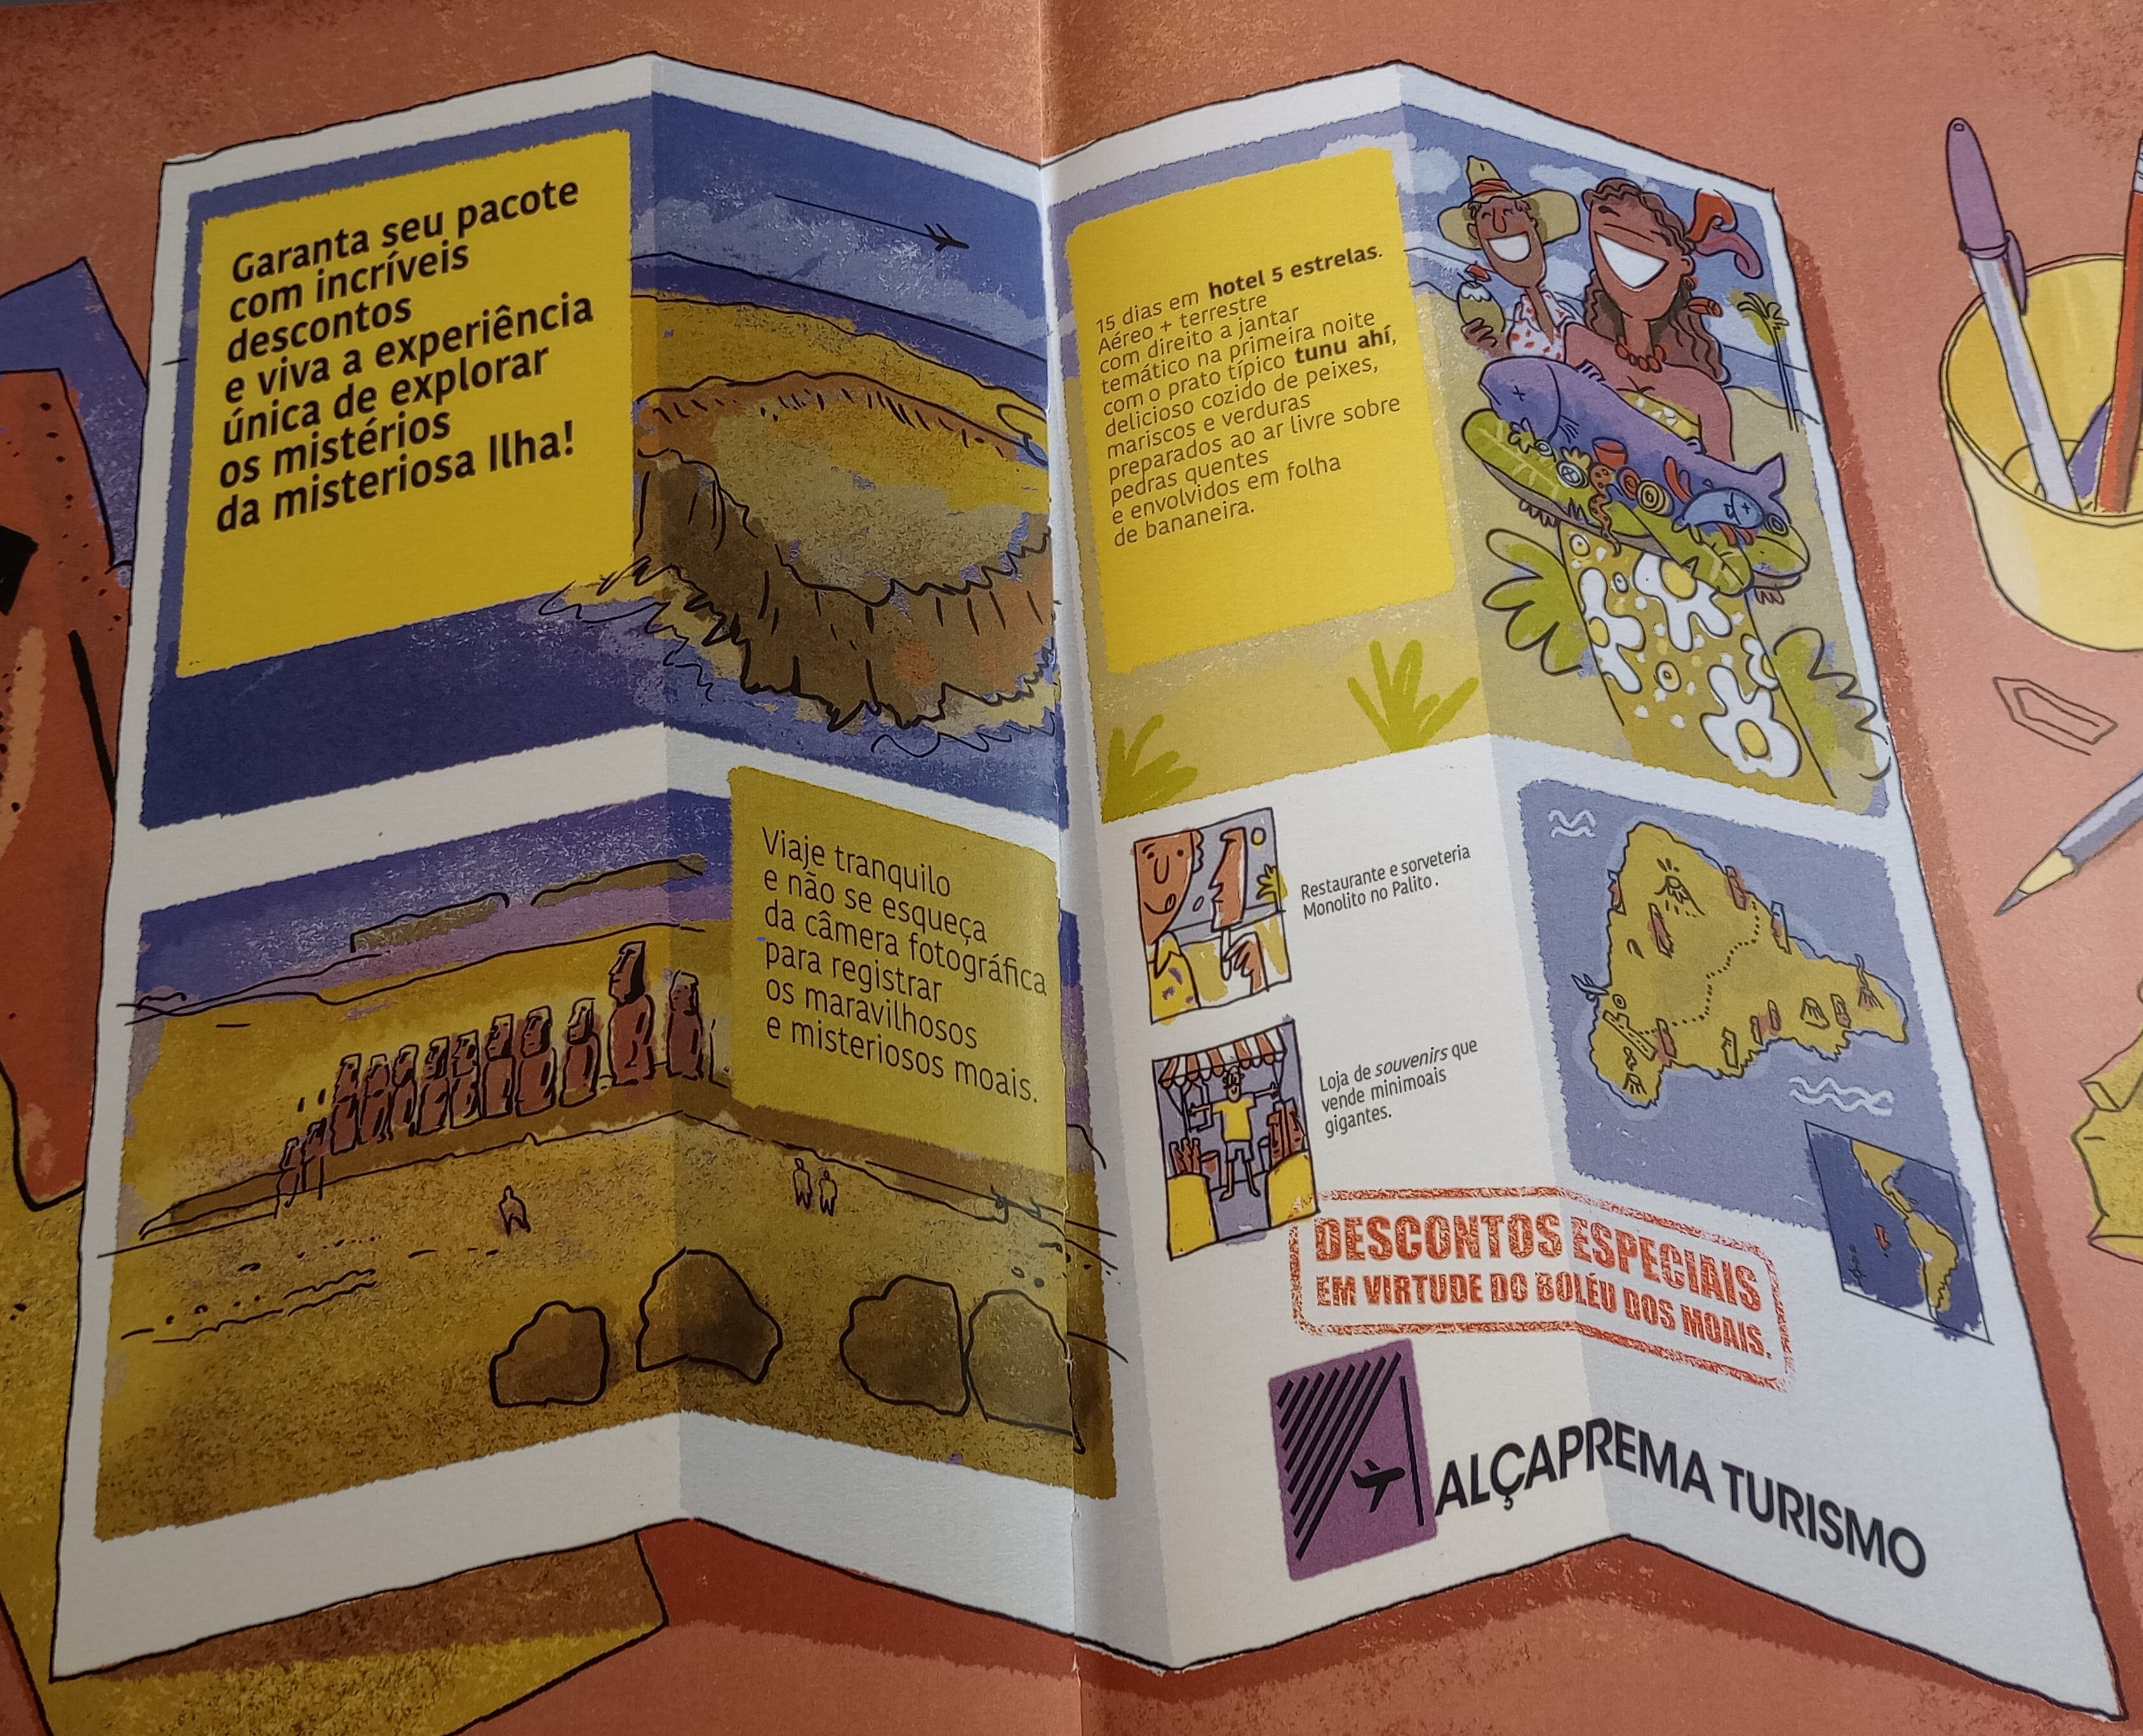
\includegraphics[width=\linewidth]{Fig1.jpeg}
    \caption{Folheto da Alçaprema Turismo}
    \label{fig1}
    \source{\textcite[p.~6-7]{franco_queda_2018}}
  \end{minipage}
\end{figure}

O \textit{folder} (\Cref{fig1}) é, aqui, emulado, como todos os demais gêneros
textuais apresentados no livro. A ilustração recria uma folha isolada, com
dobras que indicam quatro colunas, nas quais os elementos inseridos cumprem a
função publicitária: o produto divulgado é, conforme o texto aposto na parte
superior da terceira coluna, um pacote turístico que inclui “aéreo +
terrestre”, assim como “15 dias em hotel 5 estrelas” e “jantar temático na
primeira noite” \cite[p.~7]{franco_queda_2018}. Os textos, em linguagem
objetiva e breve, são reforçados pelas imagens que apresentam as maravilhas do
lugar a ser visitado, assim como pessoas felizes vivenciando a viagem, um
pequeno mapa e o logotipo da empresa. Chama a atenção um elemento acrescido ao
\textit{folder}, com as características de um carimbo aplicado a posteriori
sobre o material, no qual se lê: “Descontos especiais em virtude do boléu dos
moais” \cite[p.~7]{franco_queda_2018}.

Nas duas páginas seguintes ao \textit{folder}, o leitor acompanha uma história
em quadrinhos, na qual se utilizam as convenções dessa mídia: requadros, balões
de fala e pensamento, sarjetas. A breve narrativa apresenta uma família, com
mãe, um filho e uma filha, que presenciam a chegada do pai, que pede que todos
façam as malas, pois vão sair de férias. O anúncio é feito com as passagens na
mão, e a ele a família responde com questionamentos que revelam seus desejos: a
mãe pergunta se irão para “um chalé nas montanhas”, a filha se irão para “um
hotel fazenda cheio de bichos” e o filho se o destino é “um resort na praia com
esportes radicais” \cite[p.~8]{franco_queda_2018}. O pai responde, mostrando o
\textit{folder}, que o destino é a Ilha de Páscoa: a justificativa da escolha é
que alguma coisa acontecera no local, o que fizera com que a viagem estivesse
em promoção. À empolgação de mãe e filha com a possibilidade de férias mais
extensas, o filho responde com tristeza, a repetição da palavra “chato” (12
vezes) e uma imagem melancólica do personagem todo em azul.

As informações, fragmentadas, continuam a ser apresentadas aos leitores, e nas
páginas seguintes vemos uma reportagem, no jornal \textit{O coscuvilheiro}, com
o seguinte título: “Ascensão e queda em Rapa Nui”. Mais uma vez seguindo os
preceitos do gênero (cabeçalho com nome do veículo de comunicação, título em
caixa alta e destaque, texto em colunas, acompanhado neste caso por duas
imagens), o texto fala sobre um evento inexplicável que atingiu a Ilha de
Páscoa: a matéria começa com uma breve apresentação do local e de seus
mistérios, destacando a descoberta e documentação inaugural, em 1722, dos
moais, “essas imensas estátuas de pedra com mais de 4 metros de altura e que
podem pesar até 82 toneladas” e que são a principal atração turística da ilha.
Na sequência, a matéria informa sobre um enigma que atingiu a ilha, a queda dos
moais: “Há alguns dias, quando o sol nasceu no horizonte da Ilha, todos os
moais estavam tombados, caídos de cara no chão sem que nenhum fator climático
ou catástrofe natural tenha ocorrido para justificar essa queda”
\cite[p.~10-11]{franco_queda_2018}.

É assim que, pouco a pouco, a narrativa vai sendo articulada pela junção desses
múltiplos textos que compõem o livro. O leitor precisa se apropriar de cada um
deles, identificando sua função na composição dessa história cujo sentido só
vai se completar quando ele unir os pontos, complexamente articulados
multimodalmente. Esse movimento, conforme destaca \textcite{gibbons_i_2010} em
diálogo com estudos do campo da neurociência, envolve atividades neurais que
exigem um processamento complexo que só se efetiva mediante a co-ocorrência de
informações apresentadas pela narrativa multimodal: para o autor, nessas
narrativas “palavra e imagem atuam em sincronia, envolvidas na produção de um
significado textual compartilhado. Sua congruência narrativa é, portanto,
percebida como contribuindo para um evento conjunto”, o que implicaria que
“romances multimodais, empregando uma multiplicidade de modos, podem criar uma
experiência narrativa mais intensa” \cite[p.~101]{gibbons_i_2010}\footnote{No
original: “[…] that word and image act in synchronicity, engaged in the
production of a shared textual meaning. Their narrative congruence is thus
perceived as contributing to a joint event. Consequently, multimodal novels,
employing a multitude of modes, may create a more intense narrative
experience.”.}.

Se pensarmos que, em \textit{A queda dos moais}, além dos distintos modos,
trata-se de gêneros textuais específicos compostos para a criação da progressão
da narrativa, parece-nos que esse processo se mostra ainda mais complexo.
Afinal, é por meio da identificação desses gêneros, de suas funções e
características, que o leitor consegue reunir as informações de que necessita
para atribuir uma lógica narrativa a informações isoladas. Vejamos como isso
continua a se desenvolver na primeira parte da narrativa, o \textit{antes} da
viagem.

Após a reportagem jornalística, o próximo texto apresentado pelo livro está
composto por um \textit{e-mail}, enviado de Joaquim para a “vovó”, no qual ele
pede socorro à avó — que aparece, por meio do endereço de \textit{e-mail} a ela
atribuído, “vovó@unicalucida.dahistoria.com.br”, como alguém que o jovem julga
mais sensato que o restante da família — para evitar a viagem. É apenas nesse
momento que os personagens da história começam a ser precisados, e o garoto,
que ocupara lugar de destaque nos quadrinhos, ganha um nome. O gênero textual
fica bem marcado pela reprodução imagética de uma caixa de entrada na qual se
evidenciam os elementos que permitem sua identificação, como os endereços do
remetente e do destinatário, o assunto, o texto iniciado por um vocativo e
finalizado com uma despedida \cite[p.~110-112]{costa_dicionario_2012}, tal qual
se observa na \Cref{fig2}.

\begin{figure}[htbp]
  \centering
  \begin{minipage}{.75\textwidth}
    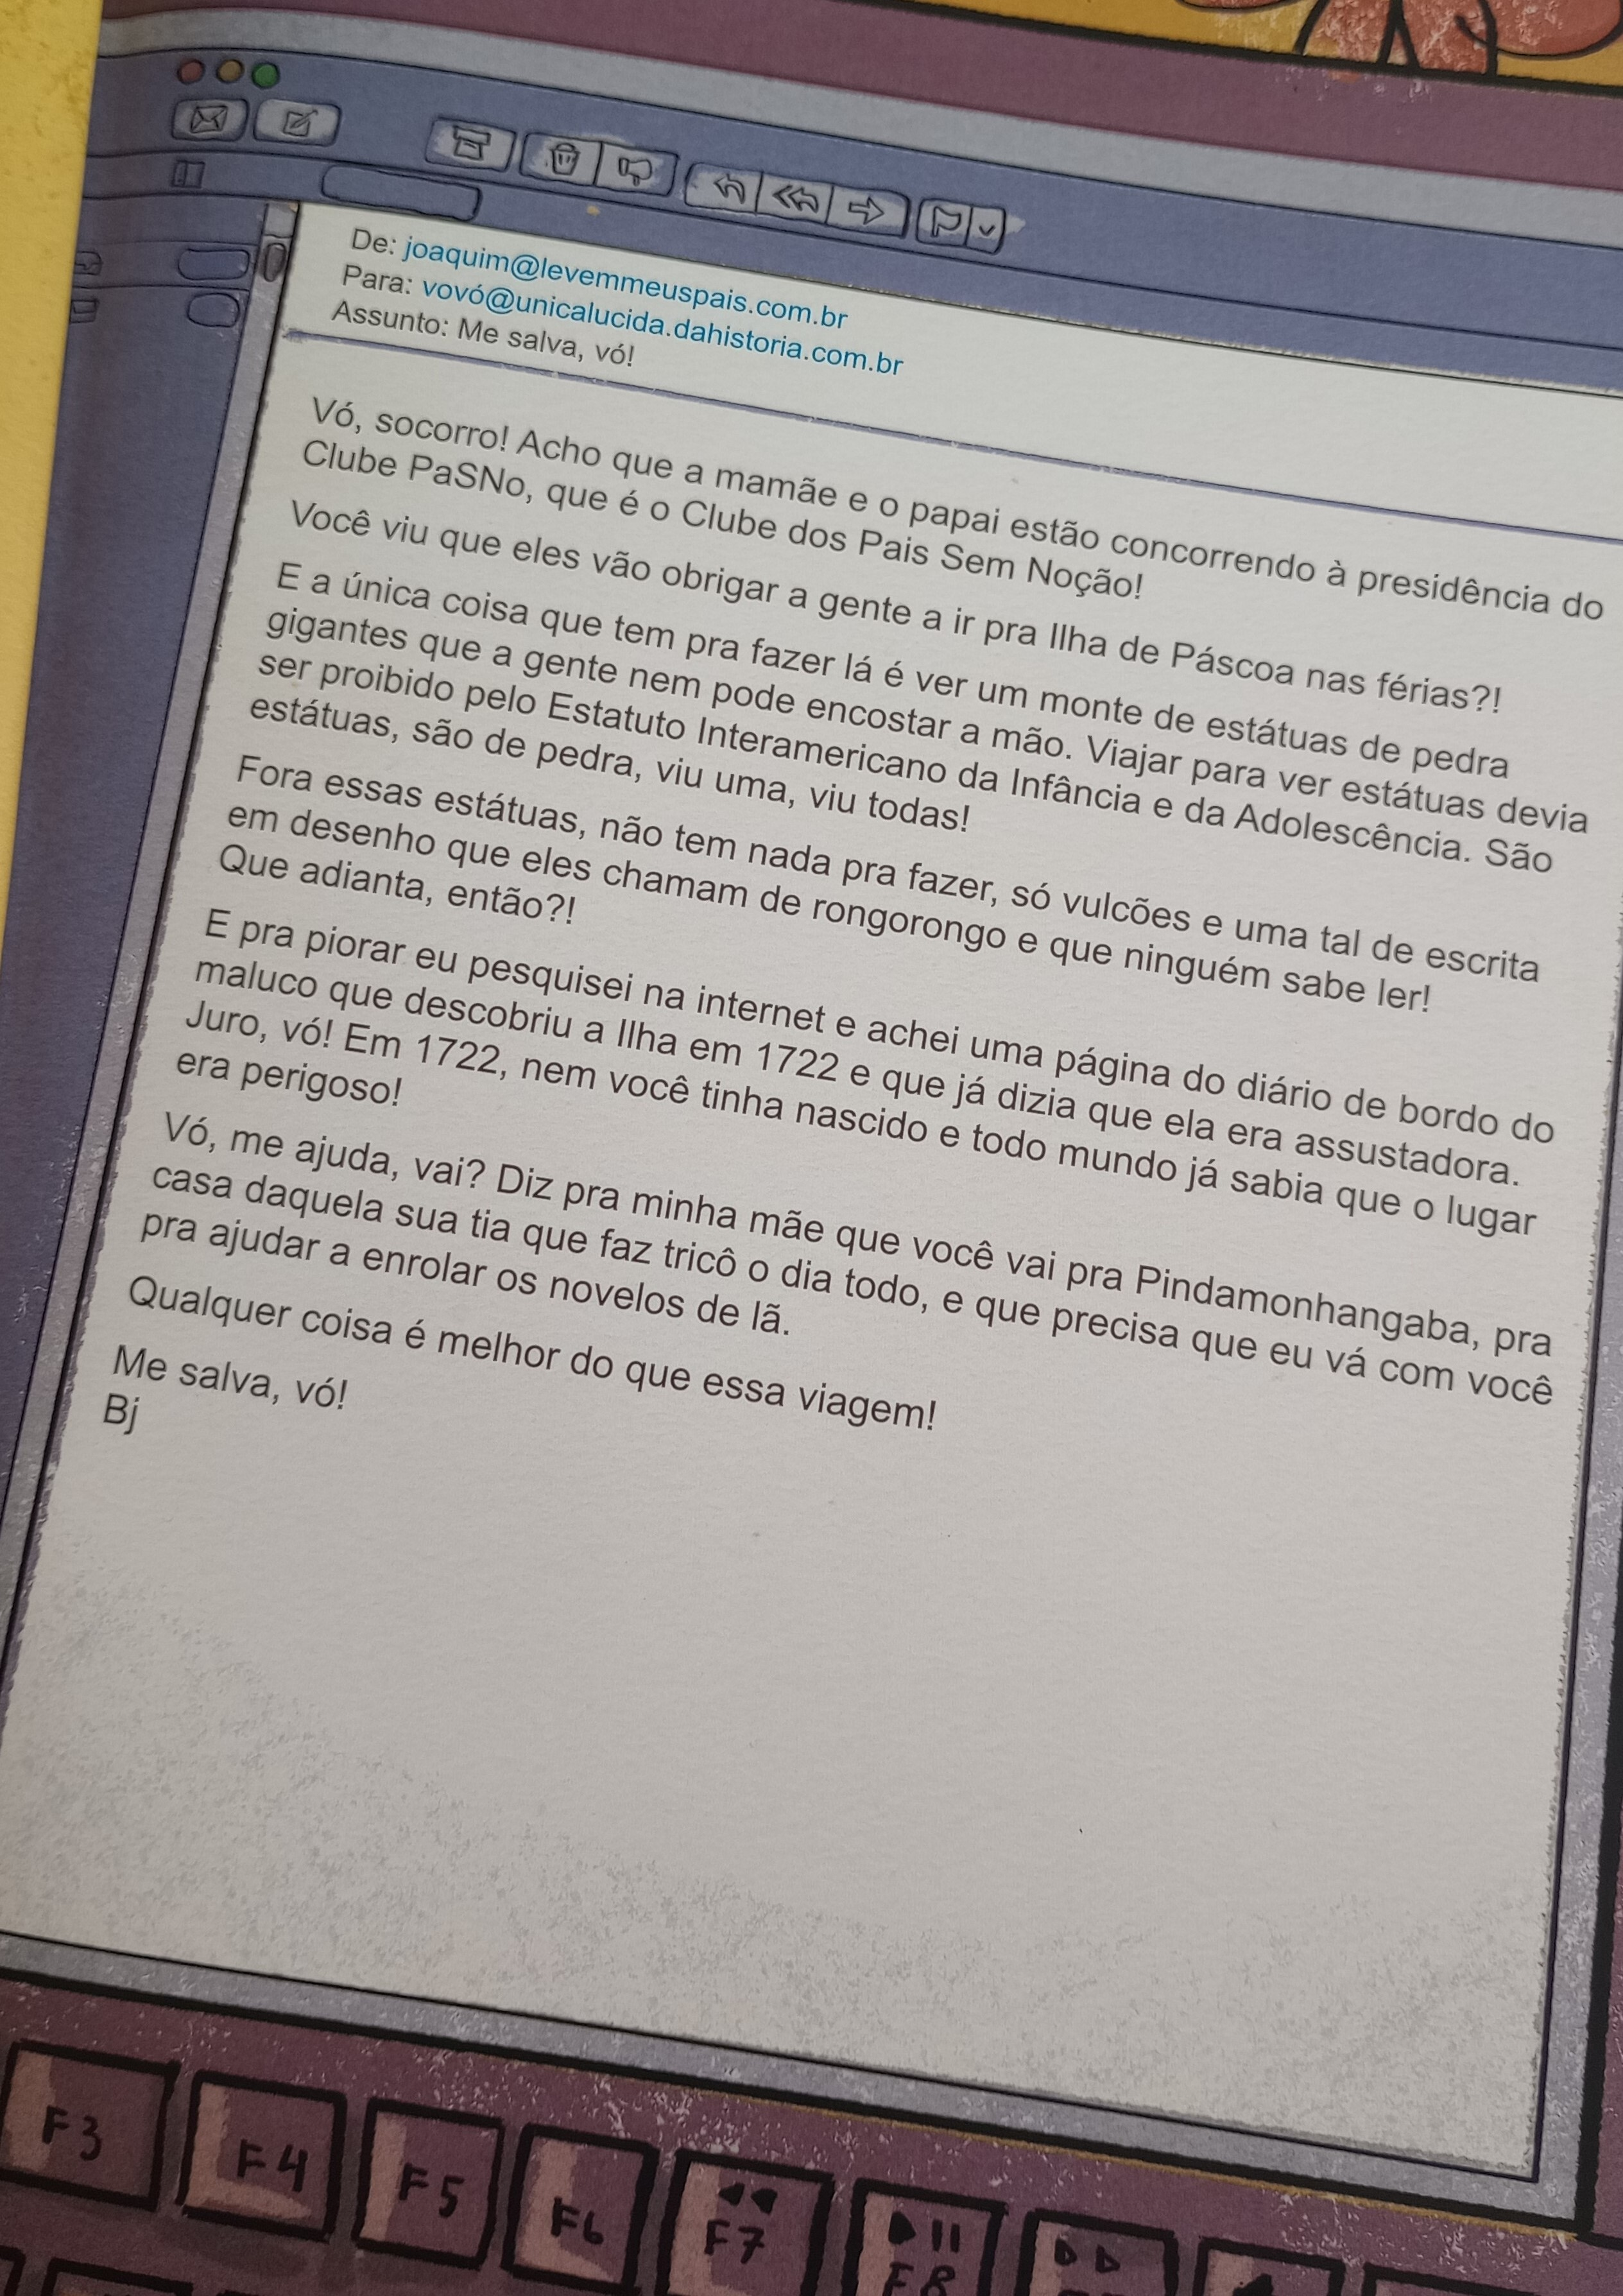
\includegraphics[width=\linewidth]{Fig2.jpeg}
    \caption{E-mail de Joaquim para sua avó}
    \label{fig2}
    \source{\textcite[p.~13]{franco_queda_2018}}
  \end{minipage}
\end{figure}

Além de pedir socorro a avó, no mesmo e-mail Joaquim informa a ela que
encontrou na internet “uma página do diário de bordo do maluco que descobriu a
ilha em 1772 e que já dizia que ela era assustadora”
\cite[p.~13]{franco_queda_2018}, e é este o texto ao qual o leitor tem acesso
nas páginas seguintes. A entrada do diário reproduzida, datada de 05 de abril
de 1722, reforça o aspecto de mistério da ilha e motiva o receio do garoto com
a viagem:

\begin{minipage}{\textwidth}
\begin{quote}
Quando nos aproximamos mais daquela ilha não assinalada em nenhum dos
nossos mapas, pudemos ver espalhadas por toda a costa as silhuetas de
vários e enormes gigantes, dispostos lado a lado pela costa, como se
\st{prontos para nos massacrar} quisessem evitar nosso desembarque.
Aconselhei o capitão a \st{fugir o mais rápido possível} ancorar em um
lugar bem distante para que, quando o sol nascesse, pudéssemos entender o
que era aquilo.

Agora é esperar que não sejamos atacados pelas criaturas maléficas que,
pressinto, habitam essa ilha.

Que Deus nos proteja! \cite[p.~15, tachados do original]{franco_queda_2018}
\end{quote}
\vspace{1em}
\end{minipage}



Esse é o último texto que encontramos na parte inicial do livro: ao virarmos a
página, nos deparamos com o mapa do \textit{durante} a viagem, e é só com esse
movimento que sabemos que as súplicas de Joaquim não funcionaram. O texto do
diário efetua o gancho narrativo, garante a situação de suspense e nos
encaminha para a Ilha de Páscoa, junto de Joaquim e sua família, com a
expectativa diante dos mistérios que ali se vivenciam. 

É, assim, por meio do diálogo entre o livro e o leitor, que precisa manejar
essas diversas textualidades, que a narrativa se encadeia e se articula: para
isso, o leitor precisa observar todos os elementos que compõem cada um dos
textos lidos, os quais ativam seus múltiplos sentidos e possibilitam a
constituição de um imaginário sensível compartilhado e multifacetado.
Certamente, a viagem de Joaquim ainda lhe guarda muitas surpresas, as quais são
também as surpresas do leitor, que precisará seguir construindo a narrativa por
meio da leitura de receitas, gráficos, piadas e relatórios, entre vários outros
gêneros, numa narrativa que, conforme apontou \textcite{lajolo_resenha_2019},
apresenta em suas pouco mais de 50 páginas algumas das características mais
marcantes da literatura contemporânea: “fragmentação da história, superposição
de linguagens, organização assimétrica das páginas”\footnote{A resenha crítica
da reconhecida pesquisadora de literatura infantil e infanto-juvenil foi
publicada no perfil do Facebook de Marisa Lajolo em 18 de abril de 2019, e
compartilhada na página de uma das autoras do livro
(\url{https://www.patriciaauerbach.com.br/mdias/marisa-lajolo-resenha-do-livro-a-queda-dos-moais}).}.
A multimodalidade independe, como vimos, de recursos tecnológicos, mas deles
também pode fazer uso para se tornar ainda mais atrativa aos jovens leitores,
como veremos a seguir.

\section{\textit{Sinfonia dos animais}}\label{sec-fmt-manuscrito}

O escritor norte-americano Dan Brown já é conhecido do grande público por obras
ficcionais que alcançaram o status de \textit{best-sellers}, responsável por
levar alguns de seus livros para as telonas. Adepto da construção narrativa em
prosa, seus romances se articulam pelo gênero suspense, estratégia ficcional
que, aliada a picos narrativos de clímax, suscita o interesse e a curiosidade
do leitor, envolvendo-o na leitura.

Por isso, chama a atenção quando Brown, já reconhecido por Hollywood e pelos
leitores de \textit{best-sellers}, busca uma renovação na estética literária
com \textit{Sinfonia dos animais}, livro publicado em 2020, sua estreia na
literatura infantil. Além de mudar o público-alvo, o escritor estadunidense
exercita outros gêneros textuais, como a poesia e a charada — esta se mescla
aos poemas, visando a uma maior aproximação com o seu leitor. A riqueza da
obra, no entanto, não se limita à pluralidade de gêneros, mas à própria
expansão da literatura, que, em \textit{Sinfonia dos animais}, é aliada da
música e das tecnologias digitais, produzindo uma experiência de leitura
multissensorial.

A conduzir os leitores pela sinfonia dos animais encontra-se o Maestro Ratinho;
é ele, inclusive, que, antes mesmo de se apresentar, na primeira página da
obra, enfatiza a estrutura especial do livro, o qual, “[...] além de olhar,
você também pode ESCUTAR” \cite[s/p, destaque do autor]{brown_sinfonia_2020}.
Assim, apontando a câmera do celular para o \textit{QR Code} presente, o leitor
poderá ler os poemas dedicados a cada um dos animais, enquanto escuta sua
sinfonia, que busca reconstituir as características e personalidades do animal
ao qual dá notas musicais. Não se trata, nesse caso, de um livro digital,
afinal é possível ler o livro de Brown sem o acesso ao \textit{QR Code}
interativo, mas, ao aliar esse recurso à leitura do livro físico, a ludicidade
ganha contornos multissensoriais. 

A literatura de Brown expande-se, cruzando as fronteiras da arte das palavras
ao buscar na estrutura musical outra forma de realização. Descobrimos, assim,
conforme nos confidencia o próprio autor ao final do livro, quando reserva umas
palavras aos seus leitores, que, muito antes de escrever histórias, ele
escrevia músicas, resgatando, portanto, uma habilidade antiga na composição de
um livro multimodal e intermídia\footnote{Segundo Claus Clüver,
“‘Intermidialidade’ é um termo relativamente recente para um fenômeno que pode
ser encontrado em todas as culturas e épocas, tanto na vida cotidiana como em
todas as atividades culturais que chamamos de ‘arte’. Como conceito,
‘intermidialidade’ implica todos os tipos de interrelação e interação entre
mídias; uma metáfora frequente aplicada a esses processos fala de ‘cruzar as
fronteiras’ que separam as mídias” \cite[p.~9]{cluver_intermidialidade_2011}.}.
Nas palavras do autor:

\begin{quote}
A música é uma espécie de narrativa, e os movimentos de orquestra em
\textit{Sinfonia dos animais}, os poemas e as ilustrações que os acompanham
trabalham em conjunto (como um \textbf{código}!) para contar uma história e
revelar algo engraçado ou interessante sobre a personalidade de algum animal.
Se você escutar com atenção, poderá encontrar cada um desses bichinhos
\textbf{escondido} na música. Além disso, cada um deles ensina uma lição,
formando uma coleção de “\textbf{segredos} para a vida” que vão ajudar você a
crescer \cite[s/p, grifos nossos]{brown_sinfonia_2020}.
\end{quote}

De maneira cifrada, tal como em uma charada, o autor aponta para outros
sentidos e outras formas de ler o seu livro para além da tradicional, ou
daquela acompanhada pela sinfonia de cada animal, quando lemos o livro seguindo
as músicas presentes no aplicativo para o qual o \textit{QR Code} nos
direciona. Essa mensagem é também anunciada pelo personagem Maestro Ratinho,
“desta grande aventura o condutor”, que, após se apresentar, revela um pouco do
jogo do livro:

\begin{quote}
Nós bolamos um plano especial\\
Pra você desvendar até o final.\\

Basta ver e escutar para achar na estrada\\
A surpresa que esconde esta jornada.\\

Busque as pistas ocultas no trajeto,\\
E então, veja só: um jogo secreto!\\
\cite[s/p]{brown_sinfonia_2020}
\end{quote}

A leitura instaura, desse modo, um jogo secreto com o leitor: este, ao
percorrer a sinfonia dos animais, sabe de antemão que há pistas ocultas,
cifradas, as quais precisa desvendar, aprisionando-o, ainda mais, nesta
aventura verbo-musical. Sobre o processo de constituição da adivinha,
\textcite{jolles_formas_1976} afirma que os gregos tinham duas palavras para
representá-la: \textit{ainigma} e \textit{griphos}. Na primeira, “está
implícito o fato do ciframento, ao passo que na segunda, que significa
propriamente ‘rede’ – a rede que nos aprisiona e cujos nós nos emaranham –
exprime-se melhor a perfídia da cifra” \cite[p.~123]{jolles_formas_1976}.

Essa parece ser a estratégia de Brown para emaranhar o seu leitor,
aprisionando-o em seus nós e garantindo sua participação ativa na leitura e na
construção do sentido do texto. Em cada página da obra dedicada a um
animal\footnote{Além do maestro Ratinho, compõem essa sinfonia o pássaro, o
canguru, o gato, a arraia, o hipopótamo, o sapo, o avestruz, o tatu, o javali,
o cavalo, a baleia, o guepardo, o elefante, o rato, o besouro, a aranha, o
morcego, o cisne e o grilo, conforme a ordem de aparição no livro.}, há letras
embaralhadas que formam uma palavra: conforme vai articulando as letras, o
leitor percebe que todas elas representam um instrumento musical. Como exemplo,
descrevamos a imagem que ilustra o poema \textit{Sapos no brejo}: há nove sapos de
diferentes tamanhos e cores. Em seus corpos, algumas letras estão camufladas, à
espera de que o leitor consiga reordená-las e formar uma palavra. No caso aqui
mencionado, as letras I, L, A, T, E, C, N, E, R formam a palavra
\textit{clarinete}. Além disso, outra regra instaurada pelo autor e pela
ilustradora Susan Batori é a dissimulação de uma abelhinha, que está sempre
escondida em um lugar inusitado e que deve ser identificada pelo leitor. No
caso de \textit{Sapos no brejo}, o inseto aparece na boca do maior sapo da imagem, um de
cor verde, como percebe-se na \Cref{fig3}.

\begin{figure}[htbp]
  \centering
  \begin{minipage}{.65\textwidth}
    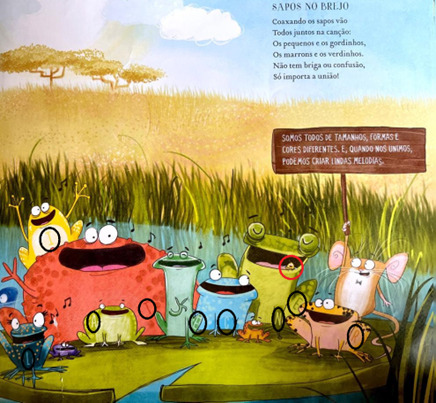
\includegraphics[width=\linewidth]{Fig3.jpeg}
    \caption{\textit{Sapos no brejo}}
    \label{fig3}
    \source{Adaptado de \textcite[s/p]{brown_sinfonia_2020}.}
  \end{minipage}
\end{figure}

Os jogos empreendidos em \textit{Sinfonia dos animais} contam, portanto, com
outras mídias: além do aplicativo de \textit{realidade aumentada} para escutar
as músicas, as imagens de Batori desempenham um papel mais complexo do que
simplesmente o de adornar um texto: afinal, elas acrescentam detalhes que não
estão presentes no poema, estabelecendo uma nova forma de o leitor se
relacionar com o livro. Exemplo disso é a existência da abelhinha que empreende
um voo pelas páginas, num jogo de ocultar-se para ser identificada pelo público
leitor.

Embora as funções tradicionalmente associadas à ilustração sejam a de adornar,
a de explicar e a de traduzir, Brown divide, em certa medida, a autoria de
\textit{Sinfonia dos animais} com Susan Batori (assim como com a orquestra que
interpreta suas músicas), porque as imagens contribuem para a construção do
sentido do texto:

\begin{quote}
Como o leitor, o ilustrador não é capaz de trazer à tona todos os significados
potenciais escondidos no texto. Ele tem de escolher entre possíveis leituras
alternativas e, ao mesmo tempo, é quase certo que fará acréscimos no texto: sua
apresentação, muito provavelmente, oferecerá informações enraizadas no mundo
visual, informações estas que o texto não consegue mediar em palavras
\cite[p.~177]{lund_historia_2012}.
\end{quote}

É justamente por não conseguir mediar todas as relações pretendidas em palavras
que o livro infantil de Dan Brown se apresenta como um texto multimodal e
intermidiático: as imagens e as músicas são convocadas para estabelecer novas
configurações e novos modos de representação, permitindo ao leitor outras
formas de conexão com a literatura, ao acessar seus cinco sentidos e sua
própria fantasia.

O ritmo e a tensão presentes na descrição do guepardo, por exemplo, só são
acessados plenamente quando o leitor permite que a sinfonia acompanhe sua
leitura, num processo que conecta os verbos \textit{ler}, \textit{ver} e
\textit{ouvir}. Na sinfonia do guepardo, o instrumento protagonista é o
violoncelo, que, num estrondo que ocorre aos 29 segundos da música, gera um
sentimento catártico no leitor, cuja expectativa havia sido alimentada pelos
primeiros segundos da música, anunciando um risco iminente. A explosão do
violoncelo torna, assim, a leitura destes versos bem mais dramática,
representando o próprio movimento empreendido pelo animal durante uma caçada,
que começa furtiva e sigilosa, tal como a música, antes de eclodir na
perseguição:

\begin{minipage}{\textwidth}
\begin{quote}
Tão furtivo e sorrateiro
    
Ele vai, leve e certeiro.

Vagaroso, lento, atento,

Não se vê um movimento.

De repente, ZÁS!

Tem início o jogo. \\
\cite[s/p, destaque do autor]{brown_sinfonia_2020}.
\end{quote}
\vspace{1em}
\end{minipage}

Esses efeitos de sentido são, portanto, não apenas assegurados como
intensificados pela relação estabelecida entre o texto e as outras mídias,
porém não podemos deixar de registrar que o autor procura também representá-los
textualmente, por meio de jogos de palavras, de rimas e de figuras de
linguagem, como a assonância e a aliteração. Esses recursos também são
responsáveis por garantir uma maior sonoridade aos poemas, e, portanto, uma
maior conexão entre literatura e música.

Diante de tamanho apuro linguístico, ressalta-se o trabalho empreendido por
Rafaella Lemos na tradução dos poemas de Brown, que, assim como o escritor
norte-americano, tenta estabelecer relações mais profundas e imediatas entre a
visão e a audição. No poema Bouncing Kangaroo, por exemplo, o autor de
\textit{O Código da Vinci} apresenta o sentido de saltitar ou quicar
(\textit{bouncing}), que marca não apenas a personalidade do animal como o seu
nome: as sílabas parecem saltitar como o mamífero, por isso elas se repetem, e
as rimas exprimem a própria sonoridade acelerada desse movimento. O
significante, assim, adquire nuances que corroboram ainda mais o sentido
pretendido, como se a relação entre o signo linguístico e o que ele representa
pudesse não ser arbitrária. Como exemplo, destacamos o verso, no original,
“Bounce to run – Ka-boing! Ka-boing!”. \textit{Boing} é uma palavra que
representa o som de algo elástico que estica e retorna à sua forma original;
figurativamente falando, descreve algo que salta, como um canguru. 

Para empreender o jogo proposto por Brown na tradução, Rafaella Lemos se vale
de outras estratégias da língua portuguesa para evidenciar linguisticamente o
salto do canguru: além da repetição de sílabas, ela recorre a uma expressão
coloquial e à referência ao folclore brasileiro – ao citar o saci – para
garantir o efeito saltitante das palavras, como em “Cangu Cangu Cangu ru, /
Pulando alto pra chuchu” e em “Pulando em bando por aí. / Pulando assim que nem
saci.”

\textit{Sinfonia dos animais} é uma obra rica de linguagens, cujos sentidos
foram apresentados e não esgotados nesta análise. A união de todos esses
elementos – a poesia, a charada, a ilustração, presentes no livro físico, e a
música, disponível pelo \textit{QR Code} –, garante uma experiência de leitura
ampliada ao livro de Brown, num processo que expande ainda mais os sentidos do
literário, borrando suas fronteiras ao reivindicar as outras artes e
tecnologias para o espaço do livro físico.

\section{\textit{Mobeybou}}\label{sec-formato}

\textit{Mobeybou} (\textit{Moving Beyond Boundaries}) é um projeto desenvolvido
por pesquisadores das mais diversas áreas da Universidade do Minho (Portugal)
que explora as novas formas de narrativa na era digital. Ora classificados como
um \textit{app book}, ora como um \textit{game}, os aplicativos já realizados
pelo projeto --
\citetitle{mobeybou_india_2023},
%\textcite{mobeybou_india_2023},
\citetitle{mobeybou_cabo_2023},
%\textcite{mobeybou_cabo_2023},
\citetitle{mobeybou_brasil_2023-3}
%\textcite{mobeybou_brasil_2023-3}
e
\citetitle{mobeybou_portugal_2023}
%\textcite{mobeybou_portugal_2023}
%\cite{mobeybou_india_2023,mobeybou_cabo_2023,mobeybou_brasil_2023-3,mobeybou_portugal_2023}
--
apresentam objetivos múltiplos, que consistem, para citar alguns deles, na
possibilidade de acompanhar personagens em suas vivências pelos países
mencionados, numa perspectiva multicultural; em acrescentar camadas
multimodais, como a voz do leitor, às narrativas, de maneira autoral (ainda que
com uma perspectiva bastante restrita); e em jogar, combatendo antagonistas,
convivendo com os animais, interagindo com e fazendo as culturas diversas
interagirem, por meio de seus elementos típicos que podem ser dispostos
concomitantemente num cenário da escolha do usuário. Por tudo isso, parece-nos
que o referido projeto é mais do que um \textit{game} ou um \textit{app book},
uma vez que promove possibilidades múltiplas de interação e de desdobramento
das propostas que contém.

Com coordenação de Cristina Sylla e financiamento da FCT – Fundação para a
Ciência e a Tecnologia e do FEDER – Fundo Europeu de Desenvolvimento Regional,
\textit{Mobeybou}, por meio de recursos pedagógicos inovadores, adéqua-se às
demandas dos usuários do século XXI, permitindo que o jovem leitor atue também
como coautor das narrativas que lê, enquanto aprende um pouco sobre a cultura
do país visitado. A escolha do papel a ser desempenhado se dá já na tela
inicial do aplicativo, na qual o usuário decide se irá jogar, ao escolher o
ícone com um controle de videogame, ou se irá conhecer a narrativa, caso opte
pelo ícone do livro aberto. 

Além desses dois ícones, há mais três: um com a cara de um animal (em
\textit{Mobeybou no Brasil}, trata-se de um tamanduá, já em \textit{Mobeybou na
Índia}, de um elefante, por exemplo), onde encontramos algumas informações
técnicas sobre o projeto; no ícone que se assemelha a páginas dispostas uma
atrás da outra, podemos escolher uma das paisagens típicas do país apresentado
e iniciar a história a partir da nossa escolha e preferência; já o último
ícone, o de um livro fechado com as letras “ABC” na capa, funciona como uma
espécie de enciclopédia, na qual o usuário consegue obter mais informações
sobre aspectos específicos da cultura do país visitado. Em \textit{Mobeybou na
Índia}, por exemplo, esse ícone apresenta mais informações sobre o encantador
de serpentes, a Índia, o pungi e o xamã, contribuindo, assim, para o processo
formativo e pedagógico do jovem leitor (\Cref{fig4}).

\begin{figure}[htbp]
  \centering
  \begin{minipage}{.85\textwidth}
    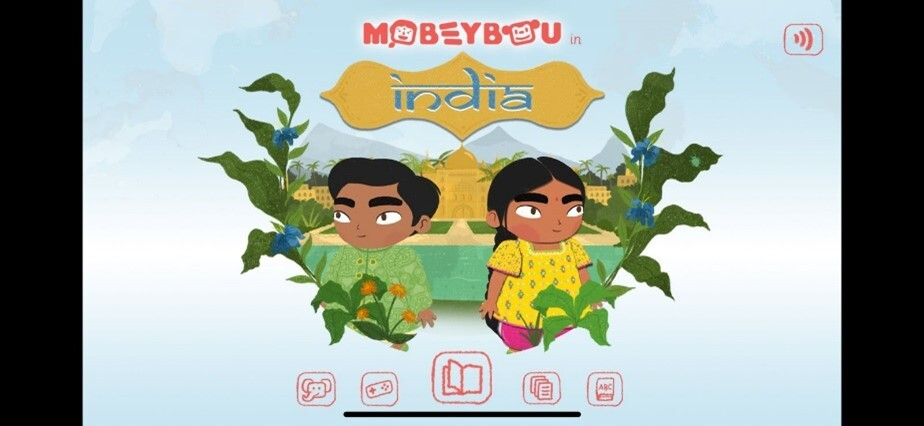
\includegraphics[width=\linewidth]{Fig4.jpeg}
    \caption{Tela inicial de \textit{Mobeybou na Índia}}
    \label{fig4}
    \source{\cite{mobeybou_india_2023}.}
  \end{minipage}
\end{figure}

Embora não apresente sofisticação estética e literária no desenvolvimento
narrativo, o projeto \textit{Mobeybou} responde às demandas da literatura
eletrônica\footnote{
    A variedade terminológica é um aspecto complexo em áreas de
    estudos recentes, como é o caso da intermidialidade ou da literatura digital.
    No Vocabulário presente no portal do Observatório da Literatura Digital
    Brasileira, da Universidade de São Carlos, os termos “literatura digital” e
    “literatura eletrônica” são tomados como equivalentes
    \cite{antunes_literatura_2024}. Mantivemos, aqui, o uso de “literatura
    eletrônica”, menos comum na América Latina que “literatura digital”, para
    preservar o léxico do artigo de Leonardo Flores com o qual dialogamos.} 
de terceira geração, conforme definição de \textcite{flores_literatura_2021}.
Partindo da classificação de N. Katherine Hayles entre literatura eletrônica de
primeira geração e literatura eletrônica de segunda geração, \textcite{flores_literatura_2021}
adiciona uma terceira. Enquanto a primeira geração da literatura eletrônica
“consiste em experiências com mídia eletrônica e digital anteriores ao advento
da rede mundial de computadores” \cite[p. 358]{flores_literatura_2021} e a
segunda, que perdura até os dias de hoje, iniciou-se com o advento da web em
1995, a terceira “utiliza plataformas estabelecidas com bases de usuários
massivas, como redes de mídia social, aplicativos, dispositivos móveis com
telas sensíveis ao toque, API e \textit{web services}”
\cite[p.~358]{flores_literatura_2021}. Assim, ainda segundo o autor, enquanto a
literatura eletrônica de segunda geração baseia-se nos critérios da tradição
literária e do mundo da arte,
\begin{quote}
[…] a literatura eletrônica de terceira geração se identifica com a mídia
eletrônica e digital tanto em seus formatos quanto em seus modelos de
publicação, produzindo trabalhos em vídeo e interativos que podem ser
publicados como videogames e outros tipos de conteúdo digital
\cite[p.~367]{flores_literatura_2021}.
\end{quote}


O projeto \textit{Mobeybou} foi concebido, assim, tal como se espera de uma
obra da literatura eletrônica de terceira geração, para leitores que, mesmo
crianças e adolescentes, já estão acostumados com as plataformas digitais,
visando responder aos anseios da cultura da internet, e não aos da tradição
artística ou literária. 

Em \textit{Mobeybou no Brasil}, por exemplo, acompanhamos a personagem Iara,
referência explícita ao folclore brasileiro, em sua viagem ao Brasil. De baixo
para cima, do sul ao norte, a primeira parada da personagem é pelos pampas
gaúchos, onde aprecia o chimarrão, bebida típica. Contempla as Cataratas do
Iguaçu para, saindo de um cenário mais natural, alcançar o agito urbano na
diversidade de São Paulo: nesse momento, a tela, em 360 graus, permite ao
usuário fazer um giro pela intensa Avenida Paulista, apreciando prédios,
museus, transeuntes e o tráfego rotineiro. 

Do sudeste ao centro-oeste, Iara chega ao Pantanal: o barulho estranho e o
movimento por trás do arbusto podem surpreender o leitor, que, ao tocar-lhe,
descobre um colorido tamanduá. A viagem cultural é entrecortada com episódios
de interação, quando a habilidade de \textit{gamer} é convocada: na tela
seguinte, Iara decide se refrescar com um suco natural; para isso, o usuário
deve levar todas as frutas até o liquidificador para que a personagem, após se
hidratar, possa retomar o percurso. E a próxima parada vem acompanhada de
música e dança: em Salvador, Iara deleita-se com a capoeira e aprende a tocar o
berimbau.

Na Floresta Amazônica, a menina percorre o rio enquanto conhece as palafitas,
para, do Amazonas ao Recife, Iara poder concluir sua viagem em ritmo de festa:
ao som do frevo, ela participa de uma festa popular que mistura tradições
africanas, indígenas e europeias. Nesse momento, o usuário pode caminhar com
Iara pelas ruas do Recife, saltando obstáculos, para que a garota cumpra seu
objetivo com êxito (\Cref{fig5}).

\begin{figure}[htbp]
  \centering
  \begin{minipage}{.85\textwidth}
    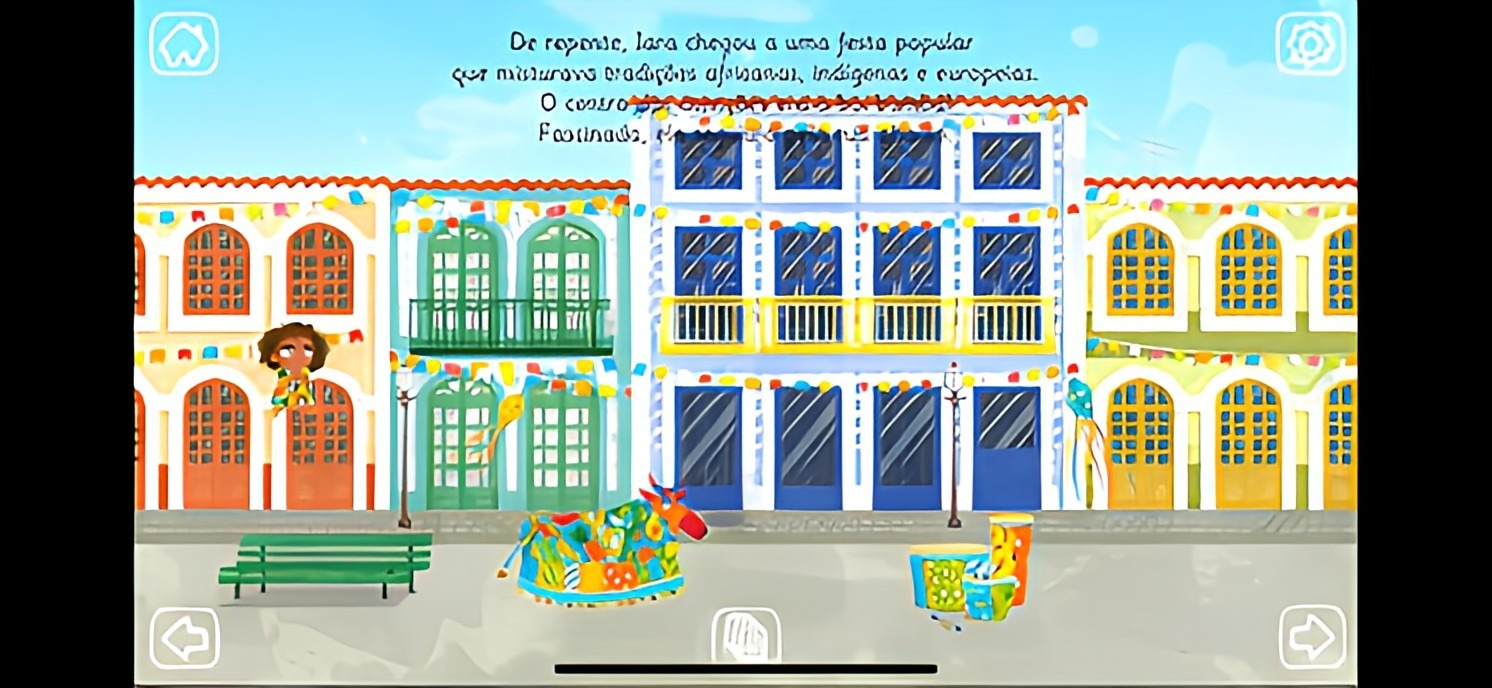
\includegraphics[width=\linewidth]{Fig5.jpeg}
    \caption{Iara em Recife}
    \label{fig5}
    \source{\cite{mobeybou_brasil_2023-3}.}
  \end{minipage}
\end{figure}

Embora o aplicativo apresente de maneira superficial a diversidade cultural e
histórica do nosso país, é um recurso interessante para que não apenas crianças
estrangeiras como também as brasileiras possam conhecer um pouco mais sobre as
raízes do Brasil. Além disso, a viagem da menina pode ser complementada com
informações adicionais presentes em uma espécie de enciclopédia, que aparece na
página inicial sob o ícone de um livro com as letras “ABC”, conforme já
mencionado.

Ainda que os recursos narrativos possam parecer muito simples, a série
\textit{Mobeybou} cria, pelo recurso multimodal associado às possibilidades
alavancadas pelas tecnologias digitais, narrativas interativas que demandam de
seus leitores um determinado grau de interação, assim como oferecem informações
de cunho intercultural que podem compor a formação desse público,
convertendo-se assim em uma experiência distinta, que, como destacou
\textcite{ellestrom_modalities_2021}, mobiliza múltiplas faculdades sensoriais
em sua realização.

\section{Considerações finais}\label{sec-modelo}

Ao longo deste artigo, buscamos refletir sobre a diversidade de formas pelas
quais a literatura contemporânea, em especial aquela endereçada a crianças e
jovens, constitui-se pelo recurso à multimodalidade. Entendemos que essa
perspectiva multimodal de construção do texto literário dialoga com um
movimento amplo que vem permeando os estudos literários mais recentemente, o
qual pontua que estamos vivenciando uma expansão do campo literário, movida por
suas facetas de produção, de leitura ou associadas à crítica.

Para tanto, selecionamos como \textit{corpus} três obras que nos parecem
contribuir para a composição desse cenário múltiplo e plural, que se valem da
multimodalidade recorrendo a diferentes estratégias. A primeira delas,
\textit{A queda dos moais}, recorre à diversidade dos gêneros textuais e ao
diálogo entre palavra e imagem, ainda que se valha apenas do formato impresso
(destaca-se que a multimodalidade não está condicionada ao digital); a segunda,
\textit{Sinfonia dos animais}, acrescenta ao diálogo verbovisual uma camada
sonora e um convite ao jogo, recorrendo ao recurso intermidiático e
incentivando a ludicidade por meio de uma mescla de tecnologias do impresso e
do digital; a última, o projeto \textit{Mobeybou}, mergulha nas potencialidades
tecnológicas, valendo-se de elementos como a gamificação e a realidade
aumentada, ainda que mantenha a imagem do livro impresso, emulado no
aplicativo.

Essa miríade de formas de se explorar os recursos multimodais origina obras
literárias que têm por fim, cada uma a sua maneira, uma exploração estética
atenta à ativação de diferentes modos de linguagem, que ultrapassam o verbal,
ainda que não deixem de a ele recorrer, e que conduzem o leitor a distintas
paisagens semióticas nas quais seus sentidos são instados a atuar, de forma
coletiva, na produção dos efeitos de sentido dos textos, os quais revelam
múltiplas e densas camadas mobilizadas. 

Não se pode negar que todas essas obras têm em comum, além da exploração
multimodal, outras duas características que nos parece relevante ressaltar. De
um lado, são obras que investem na exploração do aspecto lúdico que permeia as
narrativas e o próprio jogo do texto \cite{iser_o_1979}, reforçando elementos
de caráter interativo que demandam o envolvimento efetivo do leitor, ainda que
este ocorra em distintos graus conforme a modalidade midiática utilizada. De
outro, são obras que se mostram extremamente conscientes de sua materialidade,
e do impacto que esta tem sobre os sentidos do texto construído, reforçando
reflexões contemporâneas atinentes a esse âmbito da literatura que, muitas
vezes, foi relegado a segundo plano. 

Esperamos, portanto, ter contribuído para indicar o vigor que os estudos da
multimodalidade, associados aos da literatura em campo expandido, trazem ao
campo dos estudos literários na contemporaneidade, abrindo espaços para novos
modos de se pensar o literário mais atentos ao seu leitor, à sua materialidade
e aos múltiplos processos cognitivos a ele associados.



\printbibliography\label{sec-bib}
%conceptualization,datacuration,formalanalysis,funding,investigation,methodology,projadm,resources,software,supervision,validation,visualization,writing,review
\begin{contributors}[sec-contributors]
\authorcontribution{Maria Elisa Rodrigues Moreira}[conceptualization,writing,review]
\authorcontribution{Bruna Fontes Ferraz}
[conceptualization,writing,review]
\end{contributors}
\end{document}

